\documentclass[12pt,a4paper]{report}

\usepackage[english,russian]{babel}
\usepackage[T1,T2A]{fontenc}
\usepackage[utf8]{inputenc}
\usepackage{amsmath}
\usepackage{amssymb}
\usepackage{mathtools}
\usepackage[center]{caption}
\usepackage[caption2]{ccaption}
\usepackage{indentfirst}
\usepackage{setspace}
\usepackage{etoolbox}
\usepackage{todonotes}
\usepackage{url}

\renewcommand{\contentsname}{Содержание}
\renewcommand{\bibname}{Список литературы}
\renewcommand{\figurename}{Рис.}
\renewcommand{\tablename}{Таблица}
\renewcommand{\abstractname}{Аннотация}
\renewcommand{\partname}{Часть}

\renewcommand{\bottomfraction}{0.5}
\renewcommand{\floatpagefraction}{0.4}
\renewcommand{\textfloatsep}{0.5cm}
\renewcommand{\intextsep}{0.6cm}
\renewcommand{\floatsep}{0.3cm}

\hoffset -1.3cm
\textwidth  16.5cm
\textheight 24cm

% refs
\newcommand\figref[1]{(рис. \ref{#1})}
% for todos
\newcommand\note[1]{\textcolor{red}{(#1)}}
\newcommand\todonote[1]{\note{TODO: #1}}

\begin{document}

% Титульный лист
\begin{titlepage}
\par
\vspace*{-4cm}
\begin{center}
{\large

Санкт-Петербургский Государственный Политехнический Университет\\
Институт прикладной математики и механики\\
Кафедра прикладной математики\\

\vspace*{0.5cm}

\begin{flushright}
Диссертация допущена к защите\\
Зав. кафедрой\ \ \ \ \ \ \ \ \ \ \ \ \ \ \ \ \ \ \ \ \ \ \ \ \ \ \ \\
\underline{ \ \ \ \ \ \ \ \ \ \ \ \ \ \ \ \ \ \ \ \ \ \ \ \ \ \ \ \ \ \ \ \ \ \ \ \ \ \ \ \ \ \ \ } \\
"\underline{ \ \ \ }"\underline{ \ \ \ \ \ \ \ \ \ \ \ \ \ \ \ \ \ \ \ \ \ \ \ \ \ \ \ \ \ \ \ \ \ \ \ \ \ }
\end{flushright}

\vspace*{2.0cm}

{\Large
  \textbf{
    ДИССЕРТАЦИЯ\\
    на соискание степени МАГИСТРА\\
  }
}
\vspace*{1cm}
\textbf{
  Тема: \emph{метод ранжирования разнородных результатов поиска}\\
}

}

\vspace*{1.5cm}

\begin{flushleft}
Направление: 01.04.02 - Прикладная математика и информатика\\
Магистерская программа: системное программирование\\
\end{flushleft}

\vspace*{1cm}

Выполнил студент гр. 63601/2 \ \ \ \ \ \ \ \ \ \ \ \ \ \ \ \ \ \ \ \ \ \ \ \ \ \ \ \ \ \ \ \ \ \ \ \ \ \underline{ \ \ \ \ \ \ \ \ \ \ \ \ \ \ \ \ \ \ \ \ \ \ \ } Толмачев А.С.\\
\vspace*{0.3cm}
Руководитель, к.ф.-м.н., доц. \ \ \ \ \ \ \ \ \ \ \ \ \ \ \ \ \ \ \ \ \ \ \ \ \ \ \ \ \ \ \ \ \ \ \ \ \ \ \underline{ \ \ \ \ \ \ \ \ \ \ \ \ \ \ \ \ \ \ \ \ \ \ \ } Иванков А.А.
\vspace*{0.5cm}

\vspace*{0.3cm}

\begin{flushleft}
Консультанты:\\
\vspace*{0.3cm}
по вопросам информационного поиска \ \ \ \ \ \ \ \underline{ \ \ \ \ \ \ \ \ \ \ \ \ \ \ \ \ \ \ \ \ \ \ \ } к.ф.-м.н. Кураленок И.Е.\\
\vspace*{0.3cm}
по вопросам охраны труда \ \ \ \ \ \ \ \ \ \ \ \ \ \ \ \ \ \ \ \ \ \ \ \ \underline{ \ \ \ \ \ \ \ \ \ \ \ \ \ \ \ \ \ \ \ \ \ \ \ } к.т.н., доц. Монашков В.В.
\end{flushleft}

\end{center}
\vfill
\begin{center}
{\large Санкт-Петербург \\ 2015}
\end {center}
\end{titlepage}


\topmargin -1cm
\hoffset -0.5in
\textwidth 6.0in
\textheight 9.0in
\parindent 1cm

% 1.5 line spacing
%\renewcommand{\baselinestretch}{1.5}
\setstretch{1.5}
% Use 1.0 spacing for chapter headings
\makeatletter
\patchcmd{\@makechapterhead}{\huge}{\setstretch{1.0}\huge}{}{}
\apptocmd{\@makechapterhead}{}{}{}
\makeatother

\pagenumbering{arabic}
\setcounter{tocdepth}{4}
\normalsize

\renewcommand{\contentsname}{Содержание}
\tableofcontents

\chapter*{Введение}
\addcontentsline{toc}{chapter}{Введение}

% План:
% Мотивация
% - о важности информационного поиска и поисковых систем
% - о важности задачи ранжирования
% - о развитии поисковых систем (тренд -- внедрение результатов вертикальных поисков) + специализированные результаты для сценариев
% - о важности задачи ранжирования разнородных результатов
% Далее введение во все понятия, используемые заключении

% Важность информации в современном мире -> С развитием информационных технологий стало доступно огромное количество информации, Интернет -> надо искать в этом огромном море информации -> поисковые системы имеют очень большую важность для людей сегодня, стали неотъемлемой частью нашей жизни

C развитием информационных систем и ростом их популярности растет и количество информации, производимой с их помощью. Так, по данным аналитической компании IDC (International Data Corporation) общий объем цифровой информации в мире составил на 2013 год примерно 4.4 зеттабайт\footnote{1 зеттабайт (ЗБ) = 1 триллион гигабайт}, он увеличивается каждый год примерно на 40\% и к 2020 году составит приблизительно 44 зеттабайт \cite{IDC-Analytics}. Существенная доля этой информации -- информация, размещенная во всемирной сети Интернет. Она большей частью неструктурирована и очень разнообразна. Несомненно, без помощи поисковых систем ориентироваться в этом огромном информационном пространстве не представляется возможным. Поэтому системы веб-поиска на сегодняшний день играют очень важную роль в нашей жизни.

C момента своего возникновения веб-поисковые системы активно развиваются. Одно из современных направлений их развития касается смешивания в результатах поиска разнотипной информации. Первые системы поиска в интернете в ответ на запрос выдавали список ссылок на веб-страницы \figref{early-search-engines}.
\begin{figure}[]
  \centering
  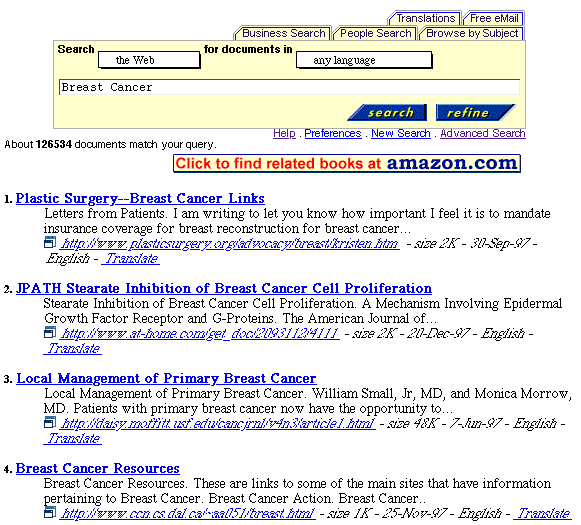
\includegraphics[height=0.33\textheight]{pics/AltavistaResults.png}
  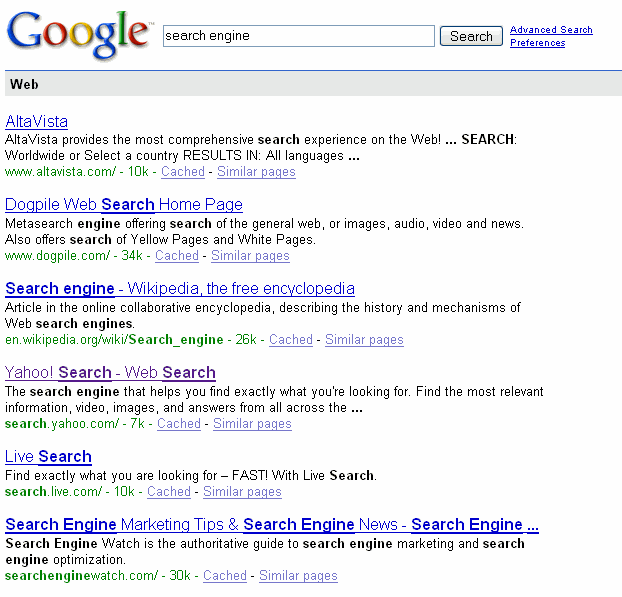
\includegraphics[height=0.33\textheight]{pics/Google-EarlyResults.png}
  \caption{Страницы результатов поиска системы AltaVista и одной из первых версий системы Google.}
  \label{early-search-engines}
\end{figure}
Такой вид результатов поиска для того времени был естественным, поскольку представляемая в них информация была однородной. 
% \note{почему?}
% поскольку информация, содержащаяся в интернете на заре его истории, не отличалась большим разнообразием. 
%Ограничение результатов поиска одним типом -- веб-страницами -- было естественным, поскольку в то время интернет по сути представлял собой набор текстовых страниц, ссылающихся друг на друга при помощи гиперссылок \note{не по этому?}. 
Но по мере того, как развивались интернет-технологии и увеличивалось число интернет-пользователей, информация, размещаемая в сети, становилось все более разнообразной. На сегодняшний день это разнообразие огромно: в интернете можно найти тексты книг, музыку, фильмы, новости, научные статьи, программные приложения, кулинарные рецепты, технические характеристики товаров и отзывы о них и т. д. -- все это различные типы информации. В связи с этим получили развитие системы, предназначенные для агрегации и поиска информации определенного типа. К таковым относятся, например, системы поиска изображений, видео-записей, новостей, товаров, музыки. Ясно, что такая специализированная система может быть более удобной и полезной для решения поисковой задачи из соответствующей области, чем система общего назначения. 
%которая на любой запрос выдает список интернет-страниц. 
Действительно, если пользователь, к примеру, ищет фотографии Дворцовой площади, то, очевидно, ему будет гораздо удобнее, если в качестве результатов поиска он будет видеть именно фотографии, а не ссылки на веб-страницы -- ему не нужно будет переходить по этим ссылкам и самостоятельно исследовать страницы в поисках фотографий.
Но выбирать каждый раз, к какой из многочисленных специализированных систем обратиться, неудобно. К тому же пользователь может не знать о существовании той или иной специализированной системы, а для каких-то поисковых задач такой системы может и не быть. Поэтому возникает естественное желание, чтобы система веб-поиска сама ``понимала'' запрос пользователя, и выдавала в ответ информацию нужного типа. Однако ограничивать ответ на запрос каким-то одним типом информации также неоправданно -- для решения своей поисковой задачи пользователю может быть полезна информация сразу нескольких типов. Так, например, при поиске информации о музыкальном исполнителе может быть полезна и его биография, и фотографии с ним, и аудио-записи исполняемой им музыки, и видео-сюжеты о нем. Или же поисковый запрос может быть многозначным -- например, по запросу ``политика'' пользователя может интересовать как информация, касающаяся самого термина, так и политические новости. 
Таким образом, более подходящим решением является смешивание результатов поиска от разных специализированных систем и представление их вместе с традиционными результатами веб-поиска -- списком ссылок на интернет-страницы. Такое смешивание мы можем наблюдать, пользуясь современными поисковыми системами. Например, в результатах поиска систем Яндекс и Google можно увидеть разнообразные специализированные результаты: на поисковый запрос о картинах -- результаты поиска по изображениям, на запрос об адресе в городе --  интерактивную карту с отмеченным адресом, на запрос о новостях -- результаты поиска по новостям, а на запрос о кафе -- специализированный ответ с найденными заведениями и информацией о них \figref{vertical-results}. 
% Такие специализированные результаты позволяют пользователю получить интересующую его информацию сразу же на странице с результатами поиска или перейти в специализированную поисковую систему и продолжить поиск информации с ее помощью.
Таким образом, результаты поиска могут быть \emph{разнородными}, поскольку могут содержать информацию разных типов.

\begin{figure}[b!]
  \centering
  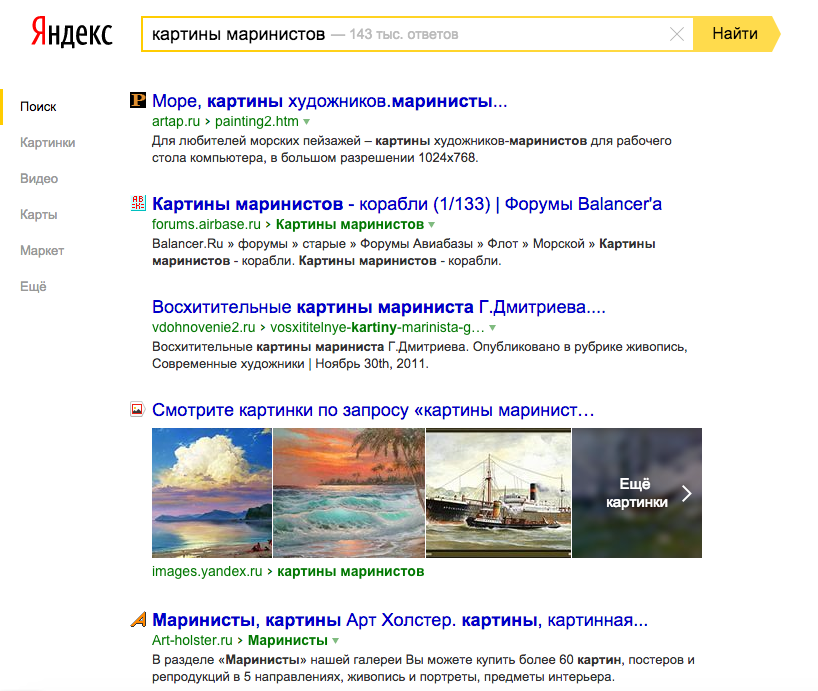
\includegraphics[height=0.3\textheight]{pics/VerticalResults-Images-Yandex.png}
  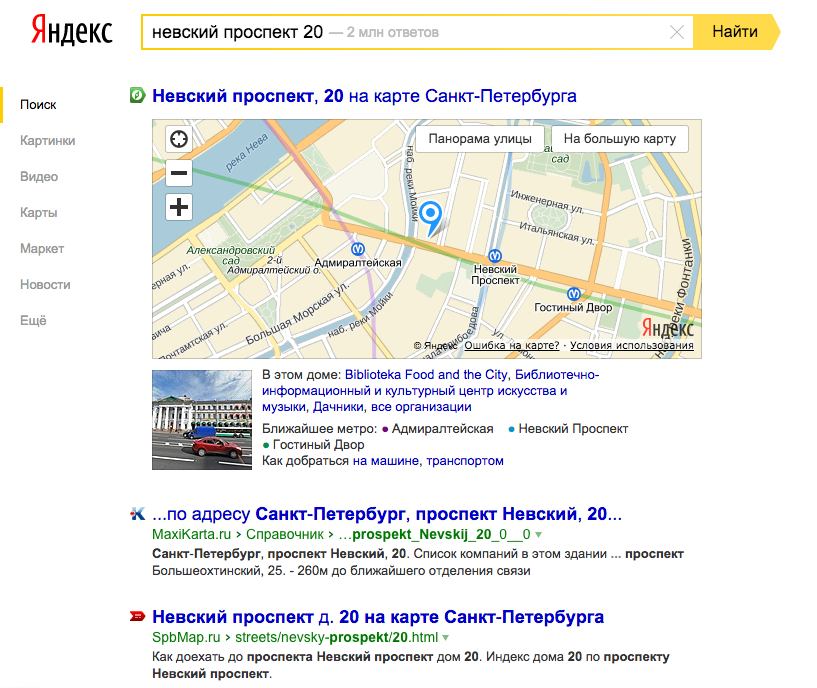
\includegraphics[height=0.3\textheight]{pics/VerticalResults-Maps-Yandex.png}
  \vfill\vfill
  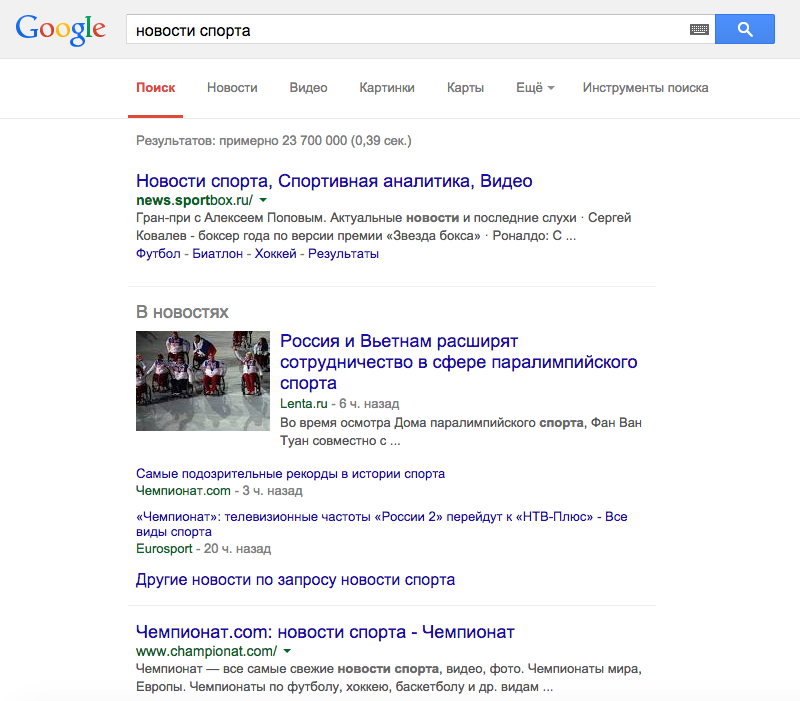
\includegraphics[height=0.3\textheight]{pics/VerticalResults-News-Google.png}
  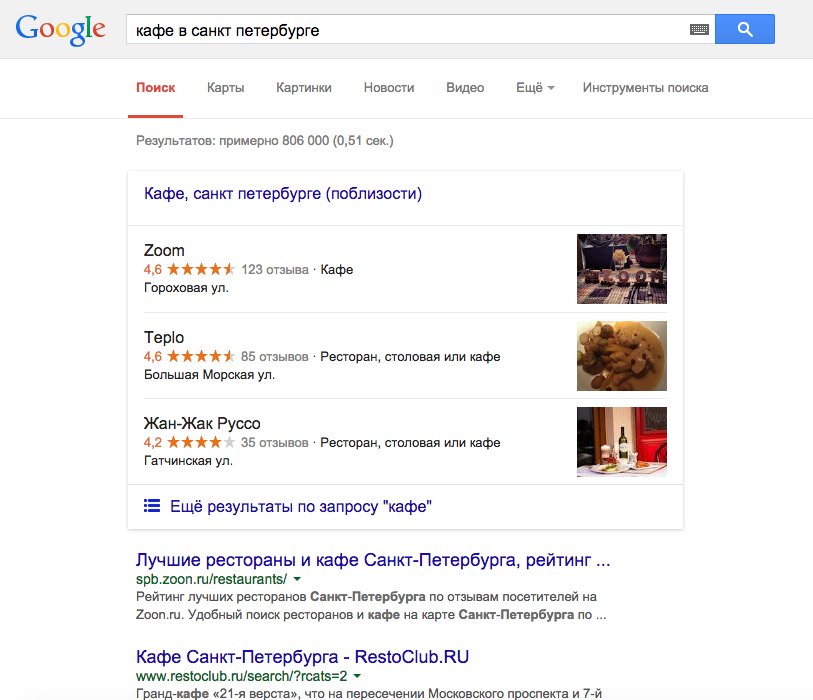
\includegraphics[height=0.3\textheight]{pics/VerticalResults-Places-Google.png}
  \caption{Специализированные ответы в результатах поиска систем Яндекс и Google.}
  \label{vertical-results}
\end{figure}

Процесс обработки поискового запроса можно условно разделить на два этапа: поиск информации, соответствующей запросу, и представление найденной информации.
На первом этапе из всего множества объектов, известных системе, выбираются те, которые по тем или иным критериям соответствуют заданному запросу. На втором этапе множество найденных объектов представляется некоторым образом и выдается пользователю. 
%Результаты поиска, представленные определенным образом, называются \emph{поисковой выдачей}. 
Задача \emph{ранжирования} относится ко второму из этих этапов. Ранжирование -- это упорядочение результатов поиска в соответствии с некоторым принципом \cite{Ashmanov, LiuLR}. От того, как упорядочены результаты, во многом зависит то, насколько успешно пользователь сможет решить свою поисковую задачу. 
%Например, если результаты представляются в виде списка, то было бы разумно стараться располагать те из них, которые могут быть наиболее полезны пользователю в контексте заданного им запроса, в начале списка, а менее полезные -- в конце.  
Так, например, если пользователь задал запрос ``скалолазание википедия'', то, вероятно, он ищет статью о скалолазании из интернет-энциклопедии Википедия. Если среди найденных результатов эта статья присутствует, то разумно расположить ее первой в списке результатов поиска, чтобы пользователь смог сразу ею воспользоваться. В противном случае ему будет сложнее найти этот результат среди остальных, а если расположить его за пределами первых десяти результатов, то он и вовсе может решить, что эта статья не была найдена.

%Представление -- это кроме оформления результатов еще и их расположение.
%То, насколько результаты будут полезны пользователю в контексте заданного им запроса, во многом зависит от того, как они расположены в поисковой выдаче. зависит от ранжирования.
% формируется \emph{поисковая выдача} -- то, что пользователь увидит как результат работы поисковой системы.

%Ранжирование -- упорядочение результатов в соответствии с некоторым принципом.
%Например, если результаты представляются в виде списка, то разумно постараться расположить наиболее полезные результаты в начале списка, а менее полезные -- в конце.

\todonote{Что-то еще о ранжировании?}

Классическая задача ранжирования формулируется для однотипных объектов.
\todonote{О классической задаче ранжирования и особенностях ранжирования разнородных результатов}

% Первые версии популярных на сегодняшний день систем Яндекс и Google  качестве результатов поиска выдавали список ссылок на интернет-страницы. 

% Взаимодействие с поисковой системой происходит следующим образом. Пользователь формулирует свою информационную потребность в виде \emph{поискового запроса} (набора ключевых слов или короткой фразы) и задает его системе. Та, в свою очередь, обрабатывает заданный запрос и выдает результаты поиска, представленные некоторым образом, -- так называемую \emph{поисковую выдачу}.

%Разумеется, пользователь ожидает, что выданные результаты будут полезны для решения сформулированной в запросе поисковой задачи.

%Процесс обработки запроса, заданного поисковой системе, можно разделить на два этапа:
%Процесс обработки запроса поисковой системой можно разделить на два этапа:
%\begin{enumerate}
%\item поиск документов, соответствующих поисковому запросу, среди ;
%\item представление найденной информации.
%\end{enumerate}

%Процесс веб-поиска можно разделить на два основных этапа:


%C момента своего возникновения веб-поисковые системы активно развиваются. Одна из современных тенденций развития веб-поиска -- встраивание в поисковую выдачу 

%Поисковые системы на заре своей истории в ответ на поисковый запрос выдавали список ссылок на интернет страницы. 

%Результаты, выдаваемые поисковыми системами на заре своей истории, представляли собой список ссылок на интернет страницы.

---------

\todonote{Это в обзор}
% Ранжирование разнородных результатов, особенности
Наиболее ранние исследования в области ранжирования разнородных результатов поиска касаются встраивания одного конкретного специализированного результата на первое место в списке результатов поиска \todonote{ссылки} и встраивания одного из нескольких специализированных результатов так же на первое место \todonote{ссылки}. Однако встраивание только одного специализированного результата на самую верхнюю позицию подходит лишь для тех случаев, когда поисковый запрос выражено относится к какой-то вертикали, и рассматриваемый специализированный результат более релевантен, чем все остальные. Однако специализированный результат может быть более или менее релевантен по сравнению с другими результатами, а также для запроса могут быть уместны одновременно несколько специализированных результатов. Поэтому более поздние исследования нацелены на встраивание специализированных результатов на различные позиции в поисковой выдаче \todonote{ссылки}. \todonote{Дописать еще}
% Но Это довольно грубое Однако зачастую 

%Традиционные методы ранжирования в информационном поиске ориентированы на ранжирование однотипных информационных объектов.  
%Современное направление -- использование методов машинного обучения для ранжирования. Проблемы при обобщении на разнородные результаты.

\begin{figure}[b!]
  \centering
  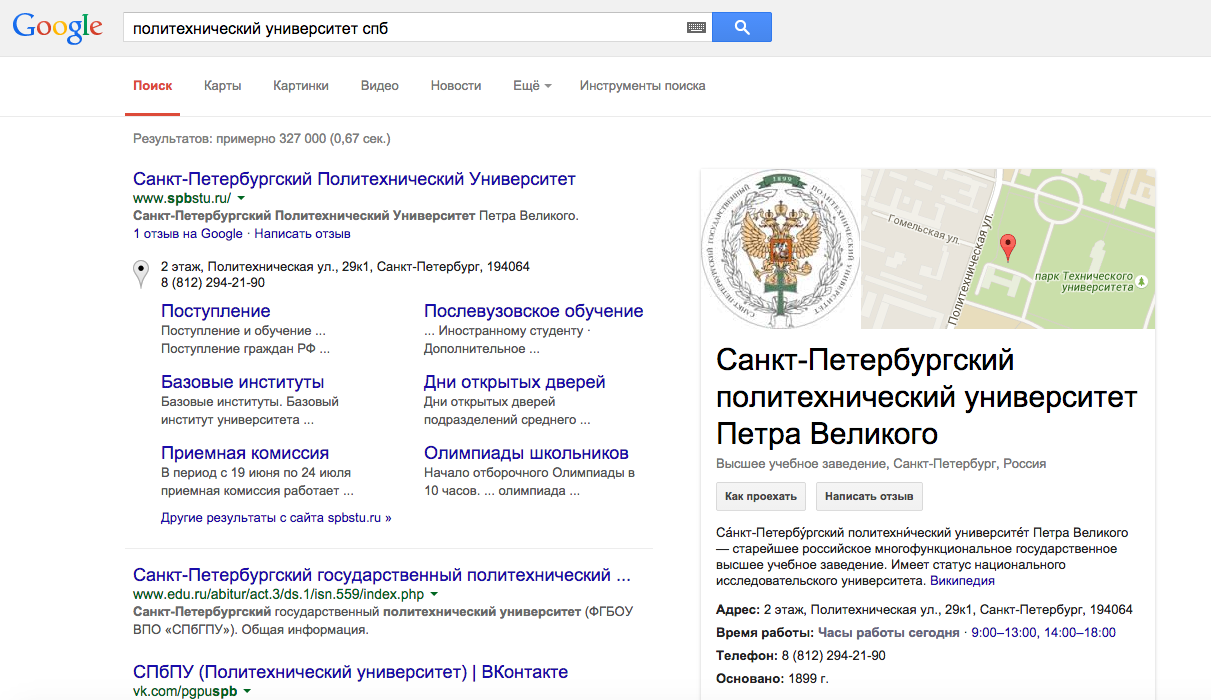
\includegraphics[width=0.9\textwidth]{pics/EntitySearch-Google.png}
  \caption{Поисковая выдача системы Google со специализированным результатом в отдельной колонке.}
  \label{two-coloumn-serp}
\end{figure}

% Разные модели поисковой выдачи, особенности, связанные с этим
Также следует отметить, что список, -- не единственный способ представления результатов поиска. Модели поисковой выдачи могут быть различными. Например, поисковая выдача системы Google для настольных компьютеров имеет две колонки, в левой из которых располагается список результатов, а в правой могут располагаться специализированные ответы \figref{two-coloumn-serp}. А выдача мобильного приложения поисковой системы Яндекс состоит из страниц, каждая из которых может содержать список результатов или специализированные ответы. Состав и порядок этих страниц может зависеть от запроса \figref{yandex-mobile-app-serp}. В таком случае задача ранжирования усложняется и превращается в задачу расположения поисковых результатов в соответствии с заданной моделью поисковой выдачи. Это также требует обобщения методов ранжирования.

\begin{figure}[t!]
  \centering
  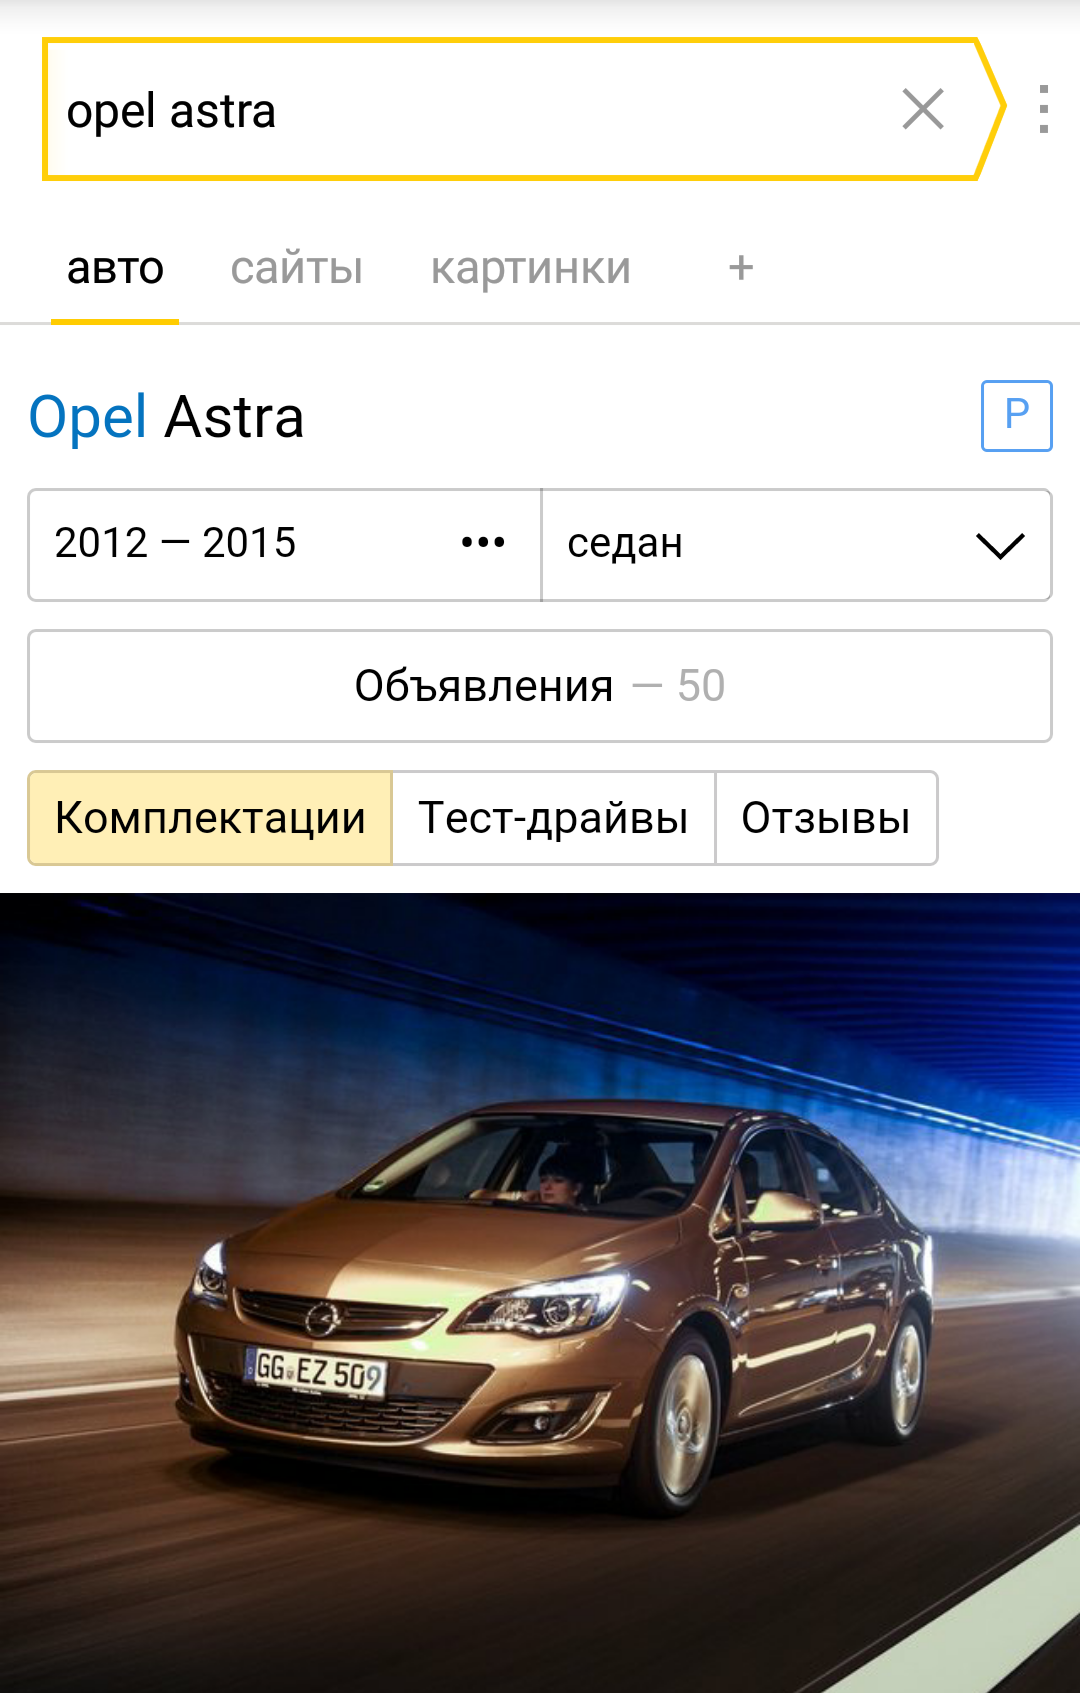
\includegraphics[width=0.3\textwidth]{pics/MultiPageSerp-Yandex-1.png}
  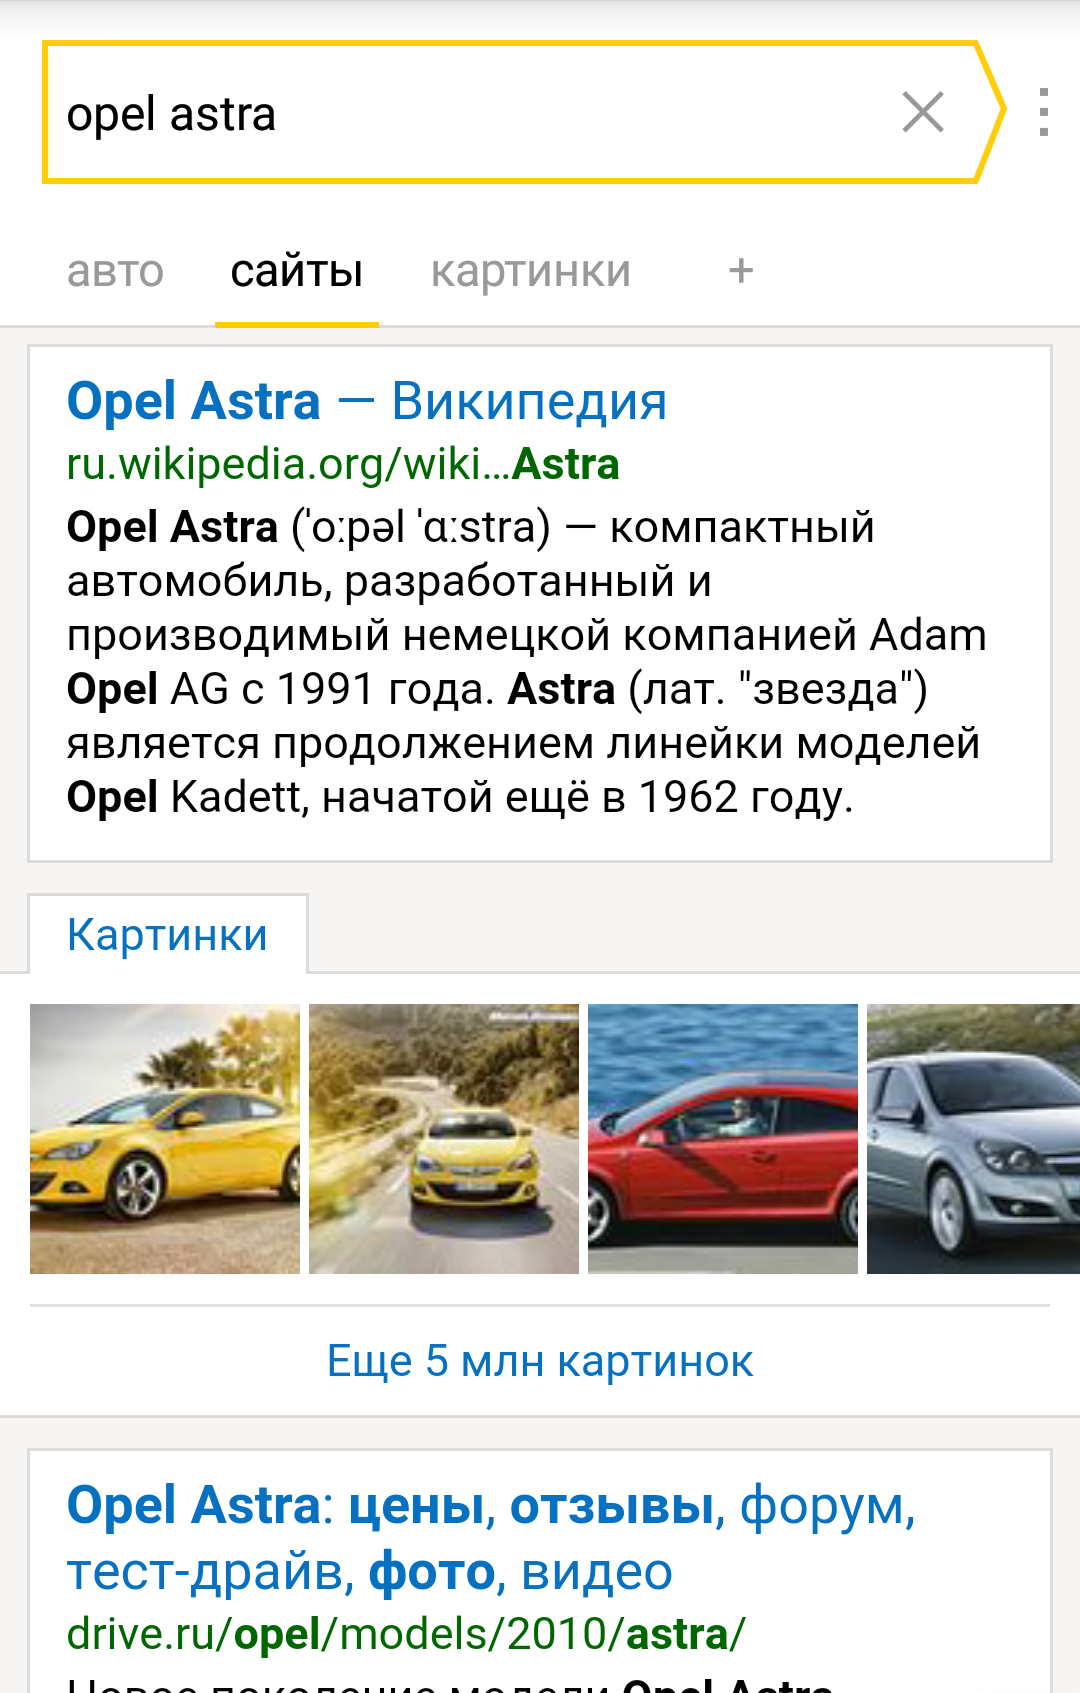
\includegraphics[width=0.3\textwidth]{pics/MultiPageSerp-Yandex-2.png}
  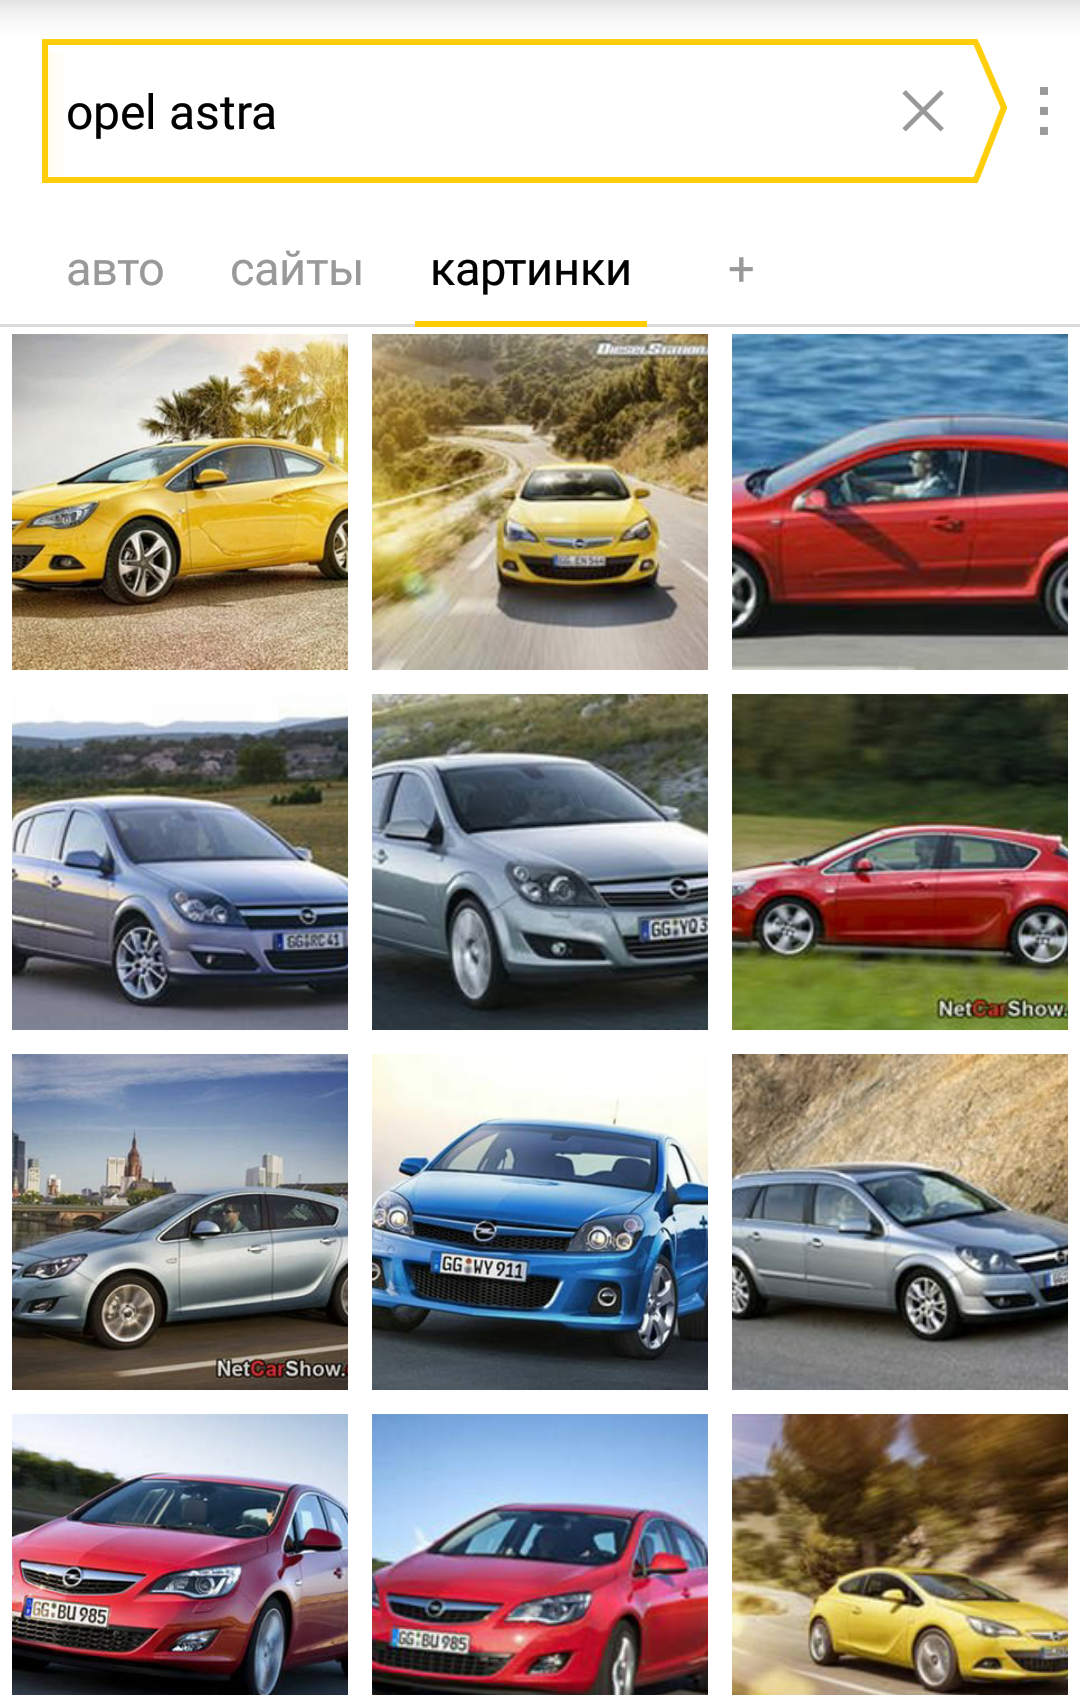
\includegraphics[width=0.3\textwidth]{pics/MultiPageSerp-Yandex-3.png}
  \caption{Выдача мобильного приложения поисковой системы Яндекс с результатами поиска на отдельных страницах.}
  \label{yandex-mobile-app-serp}
\end{figure}

%Цель поисковой системы -- сделать так, чтобы пользователь смог найти интересующую его информацию, потратив как можно меньше усилий и времени. Поэтому найденные результаты требуется расположить так, чтобы наиболее релевантные результаты были доступны пользователю в первую очередь.

%Найденные результаты требуется каким-то образом представить пользователю.  

%Совокупность результатов поиска, выдаваемых поисковой системой в ответ на запрос, представленная определенным образом называется \emph{поисковой выдачей}.

% О том, что такое результаты поиска и поисковая выдача
% Совокупность результатов поиска, выдаваемых поисковой системой в ответ на запрос, представленная определенным образом, называется ... образует \emph{поисковую выдачу}.

% О результатах подробнее 
% - о представлении результатов. список образов найденных объектов
%  - выдача -- + представление определенным образом
%  - бывают разнородными. почему

% Что-то про то, как представляются результаты
% Также большую роль играет то, как представлены найденные результаты. Результаты поиска должны быть представлены таким образом, чтобы пользователь смог найти интересующую его информацию, потратив как можно меньше усилий и времени.

% Распространенный способ представления результатов -- упорядоченный список, в котором элементы расположены по убыванию релевантности.

% Обычно результаты представляются в виде списка найденных объектов   Наиболее распространенный способ представления -- упорядоченный список найденных документов


В данной работе рассматривается задача ранжирования разнородных результатов поиска и предлагается универсальный метод ее решения. ...

%=================================================================
\chapter{Обзор литературы}

План:

\begin{itemize}
  \item Традиционная задача ранжирования, обзор методов, способов оценки
  \item Ранжирование разнородных результатов, обзор методов, способов оценки
\end{itemize}

\section{Классическая задача ранжирования}
\subsection{Формулировка задачи}
\subsection{Обзор методов решения}

\section{Задача ранжирования разнородных результатов поиска}
\subsection{Формулировка задачи}
\subsection{Обзор методов решения}

%=================================================================
\chapter{Описание метода}

\section{Основные идеи}
\section{Статистический критерий полезности поисковой выдачи}
\section{Формальная постановка задачи}
\section{Модель оценки полезности поисковой выдачи}
\section{Алгоритм ранжирования}
\subsection{Базовый алгоритм}
\subsection{``Жадный'' вариант алгоритма}

%\section{Уменьшение числа вариантов расположения результатов}

%=================================================================
\chapter{Программная реализация}

\section{Схема системы ранжирования}
\section{Уменьшение числа обращений к поисковым источникам}
\section{Используемые технологии}

%=================================================================
\chapter{Оценка качества работы метода}

\section{Методы оценки качества поиска}
\subsection{Методы, основанные на экспертных оценках}
\subsection{Методы, основанные на поведении пользователей}

\section{Выбор данных}
\section{Описание результатов}

%=================================================================
\chapter{Вопросы охраны труда}

\section{Общая характеристика санитарно-гигиенических условий труда}
\section{Эргономические требования}
\section{Микроклиматические условия}
\section{Уровень шума}
\section{Системы освещения}
\section{Излучения}
\section{Электробезопасность}
\section{Инженерно-технические мероприятия по созданию благоприятных условий труда}
\section{Методика и приборы контроля параметров среды}


%=================================================================
\chapter*{Заключение}
\addcontentsline{toc}{chapter}{Заключение}

В данной работе предложен новый метод ранжирования разнородных результатов поиска. Его отличительные особенности состоят в следующем:
\begin{itemize}
  \item ранжируемые результаты рассматриваются в совокупности, а не по отдельности;
  \item результаты располагаются в соответствии с критерием полезности, основанным на действиях пользователей на поисковой выдаче. % на странице с результатами поиска?
\end{itemize}
Благодаря этим особенностям метод обладает рядом преимуществ. Во-первых, он универсален: он может быть применен для ранжирования результатов произвольного вида и для разных моделей поисковой выдачи. Во-вторых, он позволяет естественным образом учитывать взаимосвязи между результатами. И в-третьих, он не требует экспертных оценок для обучения. 

% Какие еще преимущества?
% - легкое добавление нового типа результата / результатов от нового источника ?
% Про события, которые считаем успешными?

Предложенный метод был реализован и применен для встраивания 32-х видов специализированных результатов в поисковую выдачу системы Яндекс для мобильных устройств. Встраивались результаты поиска по изображениям, видео, мобильным приложениям, товарам, новостям, результаты гео-поиска и других сервисов компании Яндекс. 

Было оценено качество работы метода по поисковым метрикам, основанным на экспертных оценках и на поведении пользователей. В сравнении с текущим используемым методом было получено улучшение точности показа специализированных результатов на 21.22\% при снижении полноты на 29.21\% и прирост качества по метрике \textit{pfound} на 0.27\%. \todonote{уточнить результаты} \todonote{+ online-метрики}

В процессе реализации метода также была решена задача нахождения заданного числа кандидатов в аргументы максимизации значения функции, представляющей собой ансамбль ``забывчивых'' деревьев решений (oblivious decision trees), по частично вычисленному вектору признаков. Решение этой задачи позволяет избежать обращения к тем поисковым источникам, результаты которых заведомо нерелевантны заданному поисковому запросу. Разработанное решение имеет самостоятельную ценность и может быть применено и в других задачах.

\renewcommand{\bibname}{Список литературы}
\addcontentsline{toc}{chapter}{Список литературы}
\begin{thebibliography}{@}
%  \bibitem{ESL} T. Hastie, R. Tibshirani, J. Friedman. The Elements of Statistical Learning, 2nd edition. Springer, 2009.
%  \bibitem{BoostingOverview} А. Фонарев, А. Дьяконов. Обзор алгоритмов бустинга. МГУ, 2012.
%  \bibitem{MatrixNet} Алгоритм машинного обучения MatrixNet. URL: http://api.yandex.ru/matrixnet/.     
%  \bibitem{Metrics} M. Sokolova, G. Lapalme. A systematic analysis of performance measures for classification tasks. Information Processing and Management 45, p. 427–437. Elsevier, 2009.
\bibitem{IDC-Analytics} 
  International Data Corporation (IDC). The Digital Universe of Opportunities: Rich Data and the Increasing Value of the Internet of Things. // EMC website,
  URL: \url{http://www.emc.com/leadership/digital-universe/2014iview/executive-summary.htm} (дата обращения: 7.05.2015).
\bibitem{Manning-IR}
  Christopher D. Manning, Prabhakar Raghavan and Hinrich Schütze. Introduction to Information Retrieval. // Cambridge University Press. 2008. %pp. 1-3.
\bibitem{Mihalevich-CyberThesaurus}  
  Дородницын А. А. и др. Словарь по кибернетике. 2-е издание, под ред. Михалевича В.С. // Гл. ред. УСЭ им. М. П. Бажана, 1989. % C. 48.
\bibitem{Ashmanov}
  Ашманов \note{TODO}
\bibitem{SearchHistory}
  A Brief History of Search Engines. // Webreference website, 
  URL: \url{http://www.webreference.com/authoring/search_history} (дата обращения: 19.05.2015).
\bibitem{LiuLR}  
  Tie-Yan Liu. Learning to rank for information retrieval // Foundations and Trends in Informaton Retrieval, vol. 3, no. 3, pp. 225–331, 2009.
\end{thebibliography}

\chapter*{Словарь терминов}
%\addcontentsline{toc}{chapter}{Словарь терминов}

Поисковая система?

Поисковый запрос

Поисковая выдача

Поисковый источник

Специализированный ответ (специализированный результат)

Ранжирование


\end{document}


